%!TEX root = ../presentation.tex
\section{Werkzeuge}

\subsection{Workflow}
\begin{frame}{Größe}
    \begin{itemize}
        \item 103 Issues
        \item 124 Pull Requests
        \item 1243 Commits
        \item 9234 Zeilen Code
    \end{itemize}
\end{frame}

\begin{frame}{Code Reviews / Pull Reqeusts}
    \thispagestyle{plain}
    \begin{figure}
        \centering
        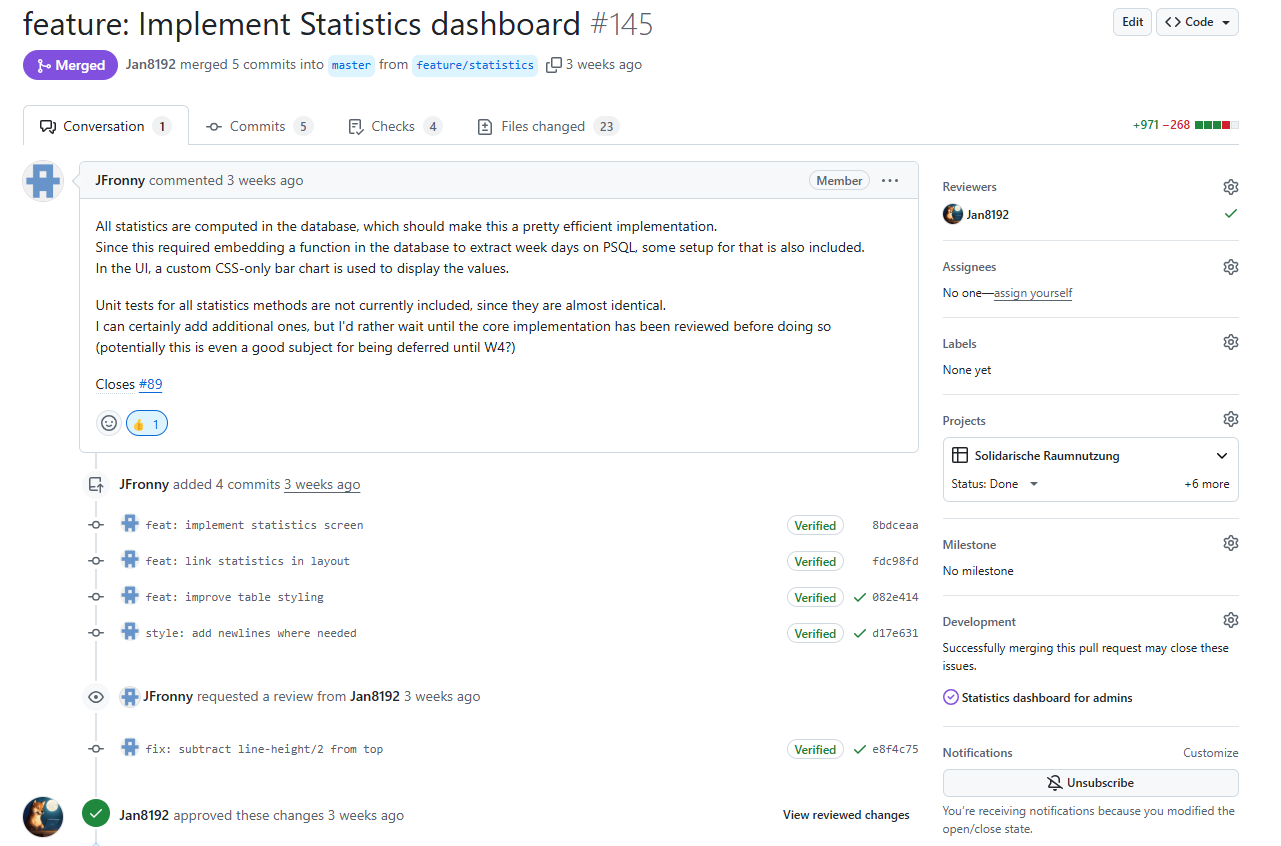
\includegraphics[width=1\linewidth]{pictures/pr_reviews}
        \label{fig:pr_reviews}
    \end{figure}
\end{frame}

\subsection{Qualität}
\begin{frame}{Unit Tests}
    \begin{columns}
        \column{.5\linewidth} \begin{itemize}
            \item 195 Unit und Integration Tests
            \item JUnit
            \item Mockito
            \item JaCoCo
        \end{itemize}
        \column{.5\linewidth} \begin{table}[h]
            \centering
            \renewcommand{\arraystretch}{1.3}
            \begin{tabular}{l|c}
                \textbf{Paket} & \textbf{Line Coverage} \\
                \hline
                \hline
                \textit{Controller}  & 77\% \\
                \textit{Domain}      & 91\%\\
                \textit{DTO}         & 83\%\\
                \textit{Filter}      & 90\% \\
                \textit{Repository}  & 100\% \\
                \textit{Service}     & 84\% \\
                \hline
                \textit{Gesamt}      & 76\% \\
            \end{tabular}
            \caption{Coverage der verschiedenen Pakete}
            \label{tab:progress}
        \end{table}
    \end{columns}
\end{frame}

\begin{frame}{CI}
    \begin{columns}
        \column{.5\linewidth} \begin{itemize}
            \item 195 Unit und Integration Tests
            \item JUnit
            \item Mockito
            \item JaCoCo
        \end{itemize}
        \column{.5\linewidth} \begin{figure}
            \centering
            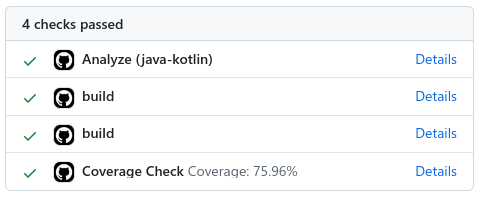
\includegraphics[width=1\linewidth]{pictures/pr_actions}
            \label{fig:pr_actions}
        \end{figure}
    \end{columns}
\end{frame}